\chapterimage{addb4870c144badba811c06724df8512.jpg}
\chapter{Anexos}
\section{Código}
\subsection{Patrón Fachada}
\begin{figure}[H]
	\centering
	\includegraphics[width=0.5\linewidth]{codfachada1}
	\centering
	\caption{Interfaz monitoría (fachada)}
	\label{fig:codfachada1}
\end{figure}
\clearpage
\begin{figure}[H]
	\centering
	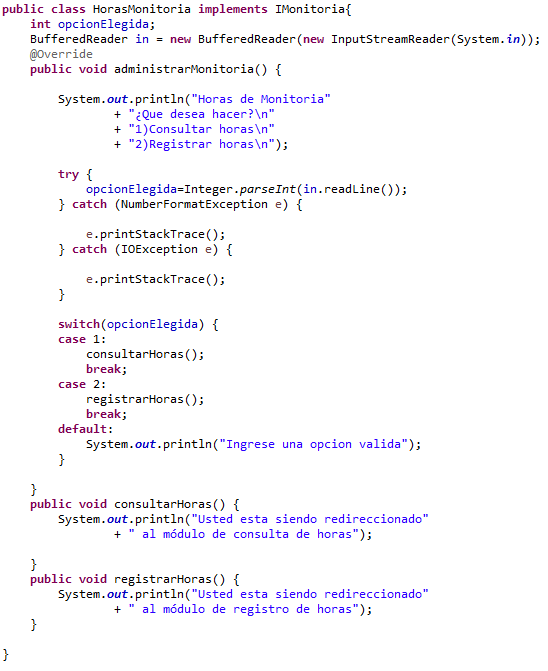
\includegraphics[width=1\linewidth]{codfachada2}
	\centering
	\caption{Ejemplo de implementación para la fachada}
	\label{fig:codfachada2}
\end{figure}
\begin{figure}[H]
	\centering
	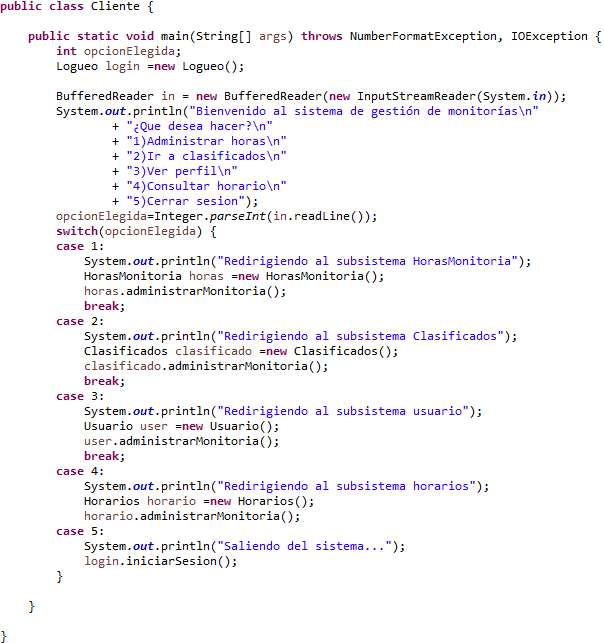
\includegraphics[width=1\linewidth]{codfachada3}
	\centering
	\caption{Cliente ejemplo fachada}
	\label{fig:codfachada3}
\end{figure}
\subsection{Patrón Proxy}
\begin{figure}[H]
	\centering
	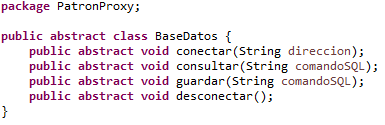
\includegraphics[width=0.5\linewidth]{codproxy1}
	\centering
	\caption{Clase abstracta de las bases de datos}
	\label{fig:codproxy1}
\end{figure}
\clearpage
\begin{figure}[H]
	\centering
	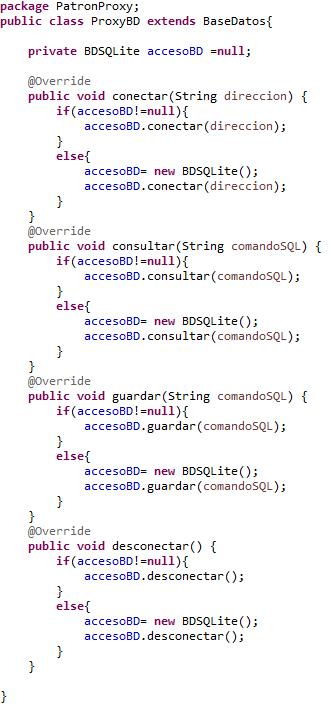
\includegraphics[width=0.7\linewidth]{codproxy2}
	\centering
	\caption{Clase proxy para el manejo de la conexión en SQLite}
	\label{fig:codproxy2}
\end{figure}
\begin{figure}[H]
	\centering
	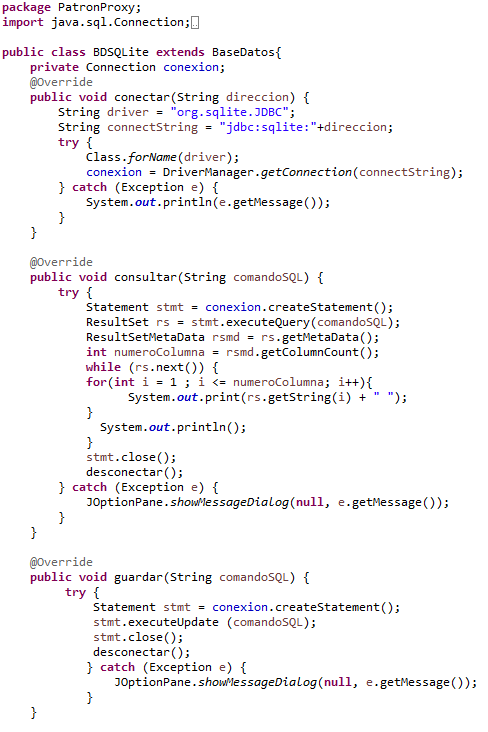
\includegraphics[width=1\linewidth]{codproxy3}
	\centering
	\label{fig:codproxy3}
\end{figure}
\begin{figure}[H]

	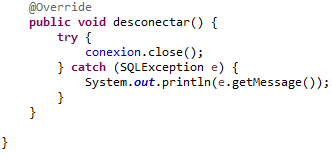
\includegraphics[width=0.7\linewidth]{codproxy4}
	\caption{Clase con la lógica de la base de datos para SQLite}

\end{figure}
\begin{figure}[H]
	\centering
	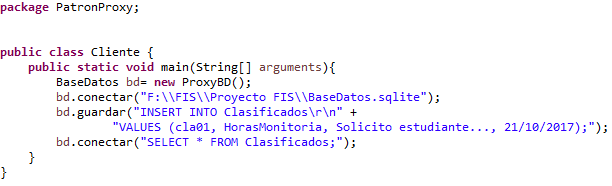
\includegraphics[width=1\linewidth]{codproxy5}
	\centering
		\caption{Cliente con un ejemplo de implementación}
	\label{fig:codproxy5}
\end{figure}

